\documentclass[UTF8,a4paper,12pt]{ctexart}
\usepackage{geometry}
\usepackage{graphicx}
\usepackage{listings}
\usepackage{xcolor}
\usepackage{tikz}
\usepackage{amsmath}
\usepackage{float}
\usepackage{hyperref}
\usepackage{booktabs}
\usetikzlibrary{shapes,arrows,positioning,automata,calc,shadows,fit}

% Optimization for line breaking and justification
\tolerance=10000
\hbadness=10000
\emergencystretch=3em
\hfuzz=1pt

\geometry{left=2.5cm,right=2.5cm,top=2.5cm,bottom=2.5cm}

\definecolor{codegreen}{rgb}{0,0.6,0}
\definecolor{codegray}{rgb}{0.5,0.5,0.5}
\definecolor{codepurple}{rgb}{0.58,0,0.82}
\definecolor{backcolour}{rgb}{0.95,0.95,0.92}

\lstdefinestyle{mystyle}{
    backgroundcolor=\color{backcolour},   
    commentstyle=\color{codegreen},
    keywordstyle=\color{magenta},
    numberstyle=\tiny\color{codegray},
    stringstyle=\color{codepurple},
    basicstyle=\ttfamily\footnotesize,
    breakatwhitespace=false,         
    breaklines=true,                 
    captionpos=b,                    
    keepspaces=true,                 
    numbers=left,                    
    numbersep=5pt,                  
    showspaces=false,                
    showstringspaces=false,
    showtabs=false,                  
    tabsize=2,
    language=Java
}

\lstset{style=mystyle}

\title{\textbf{12.3 软件组合：三叉组合树 (Trinary Combining Tree)}}
\author{trinary-combining-tree \& Trae}
\date{\today}

\begin{document}

\maketitle

\begin{abstract}
本文档仿照《The Art of Multiprocessor Programming》第12.3节的风格与结构，详细阐述了新设计的\textbf{三叉组合树 (Trinary Combining Tree)}的数据结构、实现原理及运行过程。该结构是对经典二叉组合树的扩展，通过增加节点的度数（Degree）至3，旨在降低树的高度并提高并发吞吐量。
\end{abstract}

\tableofcontents
\newpage

\section{引言 (Introduction)}
在并发编程中，单一的共享计数器（如基于CAS的\texttt{AtomicInteger}）往往成为性能瓶颈。当大量线程同时尝试更新同一内存地址时，会引发严重的内存争用（Memory Contention），导致内存总线或片上互连（On-chip Interconnect）拥塞，从而使性能急剧下降。

\textbf{软件组合（Software Combining）}技术通过将多个并发请求组织成树状结构来解决这一问题。线程从叶子节点进入，沿着路径向根节点移动。如果多个线程在同一个节点相遇，它们会将请求“合并”。其中一个线程（主动线程）继续向上携带合并后的请求，而其他线程（被动线程）则在此等待。当主动线程完成操作并返回时，它将结果分发给等待的被动线程。

本报告介绍的\textbf{三叉组合树}将每个节点的合并能力扩展为3，即每个节点最多可以汇聚3个线程的请求。相比于二叉树的 $\log_2 N$（其中 $N$ 表示并发线程数）高度，三叉树的高度降低为 $\log_3 N$，理论上能减少延迟。

\section{数据结构 (Data Structure)}

三叉组合树的核心组件是 \texttt{TriNode} 类。与二叉树节点不同，三叉节点必须能够协调最多三个线程的交互。

\subsection{节点状态 (Node Status)}
节点的状态由枚举 \texttt{CStatus3} 定义，包含以下状态：
\begin{itemize}
    \item \texttt{IDLE}: 节点处于空闲状态，无线程活动。
    \item \texttt{FIRST}: 第一个线程到达节点，暂时处于等待后续线程或准备向上移动的状态。
    \item \texttt{SECOND}: 第二个线程到达节点。
    \item \texttt{THIRD}: 第三个线程到达节点。
    \item \texttt{RESULT}: 操作已完成，结果已就绪，正在分发给被动线程。
    \item \texttt{ROOT}: 特殊状态，标识根节点。
\end{itemize}

\subsection{字段定义 (Fields)}
\texttt{TriNode} 包含以下关键字段用于同步和数据交换：

\begin{lstlisting}
public class TriNode {
    enum CStatus3 {IDLE, FIRST, SECOND, THIRD, RESULT, ROOT};
    
    boolean locked[] = new boolean[2];   // 细粒度锁控制
    int num_nodes;                       // 当前汇聚的被动线程数量
    int ready;                           // 已准备好数据的被动线程计数
    CStatus3 cStatus;                    // 当前组合状态
    
    int firstValue;                      // FIRST线程的值
    int secondValue[] = new int[2];      // SECOND和THIRD线程的值
    int result[] = new int[2];           // 分发给SECOND和THIRD的结果
    TriNode parent;                      // 父节点引用
    // ...
}
\end{lstlisting}

\begin{itemize}
    \item \texttt{secondValue[]} 和 \texttt{result[]} 数组的大小为2，分别对应 SECOND 和 THIRD 线程的数据槽位。
    \item \texttt{locked[]} 数组用于在组合协议的不同阶段协调主动线程与被动线程的步调。
\end{itemize}

\begin{figure}[H]
\centering
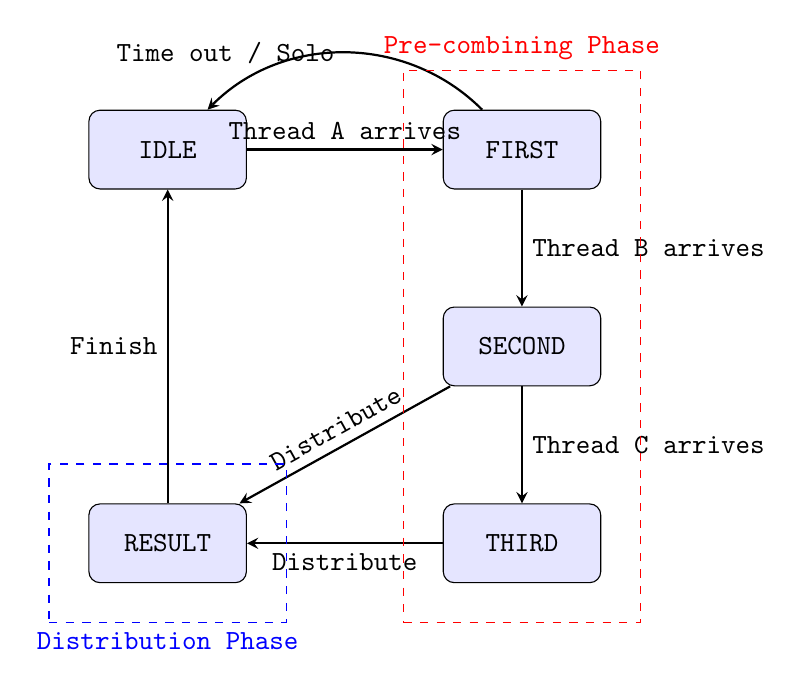
\begin{tikzpicture}[
    node distance=2.5cm,
    font=\ttfamily,
    state/.style={rectangle, rounded corners, draw=black, fill=blue!10, text centered, minimum height=1cm, minimum width=2cm},
    arrow/.style={->, >=stealth, thick}
]
    \node[state] (IDLE) {IDLE};
    \node[state, right of=IDLE, xshift=2cm] (FIRST) {FIRST};
    \node[state, below of=FIRST] (SECOND) {SECOND};
    \node[state, below of=SECOND] (THIRD) {THIRD};
    \node[state, left of=THIRD, xshift=-2cm] (RESULT) {RESULT};
    
    \draw[arrow] (IDLE) -- node[above] {Thread A arrives} (FIRST);
    \draw[arrow] (FIRST) -- node[right] {Thread B arrives} (SECOND);
    \draw[arrow] (SECOND) -- node[right] {Thread C arrives} (THIRD);
    \draw[arrow] (FIRST) to[bend right=45] node[left] {Time out / Solo} (IDLE);
    \draw[arrow] (SECOND) -- node[above, sloped] {Distribute} (RESULT);
    \draw[arrow] (THIRD) -- node[below] {Distribute} (RESULT);
    \draw[arrow] (RESULT) -- node[left] {Finish} (IDLE);
    
    % Annotated Logic
    \node[draw=red, dashed, fit=(FIRST) (SECOND) (THIRD), inner sep=0.5cm, label=above:\textcolor{red}{Pre-combining Phase}] {};
    \node[draw=blue, dashed, fit=(RESULT), inner sep=0.5cm, label=below:\textcolor{blue}{Distribution Phase}] {};
\end{tikzpicture}
\caption{TriNode 状态转换示意图}
\label{fig:states}
\end{figure}

\section{算法实现 (Algorithm Implementation)}

三叉组合树的协议分为四个阶段：预合并 (Pre-combining)、合并 (Combining)、操作 (Operation) 和 分发 (Distribution)。入口方法为 \texttt{getAndIncrement()}。

\subsection{第一阶段：预合并 (Pre-combining)}
线程首先根据 \texttt{ThreadID} 映射到叶子节点，然后调用 \texttt{precombine()}。该方法决定了线程的角色（FIRST, SECOND 或 THIRD）。

\begin{lstlisting}
synchronized boolean precombine() throws InterruptedException {
    while (locked[1] || num_nodes >= 2) wait(); // 等待上一轮清理或名额空缺
    switch (cStatus) {
        case IDLE:
            cStatus = CStatus3.FIRST;
            return true; // 成为主动线程
        case FIRST:
            locked[0] = true; // 锁定，阻止FIRST过早进行combine
            num_nodes = 1;
            cStatus = CStatus3.SECOND;
            return false; // 成为被动线程
        case SECOND:
            num_nodes = 2;
            cStatus = CStatus3.THIRD;
            return false; // 成为被动线程
        // ...
    }
}
\end{lstlisting}
\begin{itemize}
    \item \textbf{FIRST}: 返回 \texttt{true}，表示它将作为主动线程继续向上。
    \item \textbf{SECOND/THIRD}: 返回 \texttt{false}，它们将在后续的 \texttt{op()} 方法中等待。
    \item 注意 \texttt{locked[0] = true}：这是 SECOND 线程设置的，用于通知 FIRST 线程“有同伴到了，请稍等我准备数据”。
\end{itemize}

\subsection{第二阶段：合并 (Combining)}
主动线程（FIRST）在向上移动前，调用 \texttt{combine()} 来收集被动线程的值。

\begin{lstlisting}
synchronized int combine(int combined) throws InterruptedException {
    // 等待被动线程准备好 (locked[0]被清除 且 ready数达标)
    while (locked[0] || ready < num_nodes) wait(); 
    
    locked[1] = true; // 锁定后续，防止新一轮干扰
    firstValue = combined;
    
    switch (cStatus) {
        case FIRST: return firstValue; // 无人合并
        case SECOND: return firstValue + secondValue[0]; // 合并1个
        case THIRD: return firstValue + secondValue[0] + secondValue[1]; // 合并2个
        // ...
    }
}
\end{lstlisting}
主动线程在此处计算局部子树的总和（Prefix Sum），准备携带该总和向父节点进发。

\subsection{第三阶段：操作 (Operation)}
这是协议的关键交互点。
\begin{itemize}
    \item \textbf{主动线程}: 到达树的顶端（或某个中间节点停止点）执行实际的加法操作，或者从父节点获取结果。
    \begin{itemize}
        \item \textbf{“到达树的顶端（或某个中间节点停止点）”}：对应 \texttt{TriTree.java} 中 \texttt{getAndIncrement} 方法的第一阶段循环。如果 \texttt{precombine()} 返回 \texttt{true}（状态 IDLE $\rightarrow$ FIRST），线程继续向上；如果返回 \texttt{false}（遇到非空闲节点或根节点），线程停止上升，该节点即为停止点 \texttt{stop}。
        \item \textbf{“执行实际的加法操作，或者从父节点获取结果”}：对应 \texttt{TriNode.java} 中 \texttt{op()} 方法的分支逻辑。如果停止点是 \texttt{ROOT}，线程执行全局加法（\texttt{result += combined}）；如果停止点是中间节点（此时线程在该节点角色为 SECOND 或 THIRD），它进入等待状态（\texttt{wait()}），直到父节点的主动线程完成操作并分发结果。
    \end{itemize}
    \item \textbf{被动线程}: 调用 \texttt{op()} 实际上是进入等待状态，并向主动线程提交数据。
\end{itemize}

被动线程在 \texttt{op()} 中的逻辑：
\begin{lstlisting}
// 在 TriNode.java 的 op() 方法中
case SECOND:    
case THIRD:
    int myIndex = ready;
    secondValue[myIndex] = combined; // 提交自己的值
    ready++;
    if (ready >= num_nodes) {
        locked[0] = false; // 所有被动线程就绪，释放锁，允许FIRST继续
        notifyAll();
    }   
    while (cStatus != CStatus3.RESULT) wait(); // 等待结果
    // ... 获取结果并返回
\end{lstlisting}

\subsection{第四阶段：分发 (Distribution)}
当主动线程拿到最终结果（\texttt{prior}）后，它在回程路上调用 \texttt{distribute()} 将结果分发给被动线程。

\begin{lstlisting}
synchronized void distribute(int prior) throws InterruptedException {
    switch (cStatus) {
        case SECOND:
            result[0] = prior + firstValue; // 分发给SECOND
            cStatus = CStatus3.RESULT;
            break;
        case THIRD:
            result[0] = prior + firstValue; // 分发给SECOND
            result[1] = result[0] + secondValue[0]; // 分发给THIRD
            cStatus = CStatus3.RESULT;
            break;
        // ...
    }
    notifyAll(); // 唤醒等待的被动线程
}
\end{lstlisting}
这里实现了结果的\textbf{序列化}。假设 FIRST 增加 $v_1$, SECOND 增加 $v_2$, THIRD 增加 $v_3$。
\begin{itemize}
    \item FIRST 得到 \texttt{prior}。
    \item SECOND 得到 \texttt{prior} + $v_1$。
    \item THIRD 得到 \texttt{prior} + $v_1$ + $v_2$。
\end{itemize}
这确保了所有线程虽然是并发执行，但获得的返回值是连续且唯一的，就像它们排队执行一样。

\section{运行过程示例 (An Execution Trace)}

假设有线程 A, B, C 同时到达同一个节点 $N$，且都试图增加 1。

\begin{enumerate}
    \item \textbf{Arrival}: 
    \begin{itemize}
        \item A 到达，见状态 IDLE，变为 FIRST，返回 \texttt{true}。
        \item B 到达，见状态 FIRST，变为 SECOND，设置 \texttt{locked[0]=true}，返回 \texttt{false}。
        \item C 到达，见状态 SECOND，变为 THIRD，返回 \texttt{false}。
    \end{itemize}
    
    \item \textbf{Coordination}:
    \begin{itemize}
        \item A 调用 \texttt{combine()}，发现 \texttt{locked[0]} 为 true，\textbf{等待}。
        \item B 进入 \texttt{op()}，写入 \texttt{secondValue[0]=1}，\texttt{ready} 变为 1。
        \item C 进入 \texttt{op()}，写入 \texttt{secondValue[1]=1}，\texttt{ready} 变为 2。此时 \texttt{ready == num\_nodes}，C 设置 \texttt{locked[0]=false} 并 \texttt{notifyAll()}，然后 B 和 C 等待结果。
    \end{itemize}
    
    \item \textbf{Combination}:
    \begin{itemize}
        \item A 被唤醒，检测到锁释放且人齐了。
        \item A 计算总和：$1 (\text{A}) + 1 (\text{B}) + 1 (\text{C}) = 3$。
        \item A 携带 3 继续向上遍历。
    \end{itemize}
    
    \item \textbf{Operation}:
    \begin{itemize}
        \item A 到达根节点（假设当前根的值为 10），执行加法 $10 + 3 = 13$。
        \item A 获得返回值 10（这是 A 的返回值）。
    \end{itemize}
    
    \item \textbf{Distribution}:
    \begin{itemize}
        \item A 回到节点 $N$，调用 \texttt{distribute(10)}。
        \item 计算 B 的结果：$10 + 1 = 11$。
        \item 计算 C 的结果：$11 + 1 = 12$。
        \item 状态设为 RESULT，唤醒 B 和 C。
    \end{itemize}
    
    \item \textbf{Completion}:
    \begin{itemize}
        \item A 返回 10。
        \item B 醒来，读取 11，返回。
        \item C 醒来，读取 12，返回。
    \end{itemize}
    最终计数器从 10 变为了 13，三个线程分别得到了 10, 11, 12，完全正确。
\end{enumerate}

\section{分析 (Analysis)}

\subsection{正确性 (Correctness)}
三叉组合树保证了线性一致性（Linearizability）。通过在节点处的各种锁机制（\texttt{locked[]}）和状态机转换，确保了：
1. 主动线程不会在被动线程数据未就绪时离开。
2. 被动线程不会在未收到结果时离开。
3. 结果的分发严格遵循前缀和逻辑，保证返回值的唯一性和连续性。

\subsection{性能 (Performance)}
设 $P$ 为处理器（线程）数量。
\begin{itemize}
    \item \textbf{树高}: 三叉树的高度为 $\lceil \log_3 P \rceil$，而二叉树为 $\lceil \log_2 P \rceil$。例如，当 $P=64$ 时，二叉树高 6 层，三叉树仅需 4 层。
    \item \textbf{延迟}: 在无争用情况下，延迟与树高成正比。三叉树减少了路径长度，理论上延迟更低。
    \item \textbf{吞吐量}: 在高争用情况下，每个节点一次能处理 3 个请求，比二叉树的 2 个请求具有更高的并行聚合能力。
    \item \textbf{空间开销}: 节点结构稍微复杂，增加了数组字段，但节点总数减少（约为二叉树的 $2/3$）。
\end{itemize}

综上所述，三叉组合树在保持软件组合技术优势（减少热点争用）的同时，通过增加节点的扇出（Fan-out），进一步优化了大规模并发场景下的延迟和吞吐量表现。

\end{document}
